\documentclass[10pt,twocolumn,letterpaper]{article}

\usepackage{cvpr}
\usepackage{times}
\usepackage{epsfig}
\usepackage{graphicx}
\usepackage{amsmath}
\usepackage{amssymb}

% Include other packages here, before hyperref.

\usepackage[breaklinks=true,bookmarks=false]{hyperref}

\cvprfinalcopy

\def\httilde{\mbox{\tt\raisebox{-.5ex}{\symbol{126}}}}

\begin{document}

\title{Geneus: An Enigma of Organism Intelligence}

\author{Jason Dong, Yidi Huang, Mark Lalor, Andrew Tarnoff, Hung Vu \\
Case Western Reserve University\\
10900 Euclid Ave, Cleveland, OH 44106\\
{\tt\small jwd67@case.edu, yxh597@case.edu, mwl58@case.edu, art81@case.edu, hdv4@case.edu}}

\maketitle

\begin{abstract}
   This will be teh abstract which will be wonderfully descriptive yet succinct.
\end{abstract}

\section{Introduction}

This is the introduction \cite{Alpher02}

\section{Background}

This is the background \cite{Alpher04}

\section{Data}

\begin{figure}
  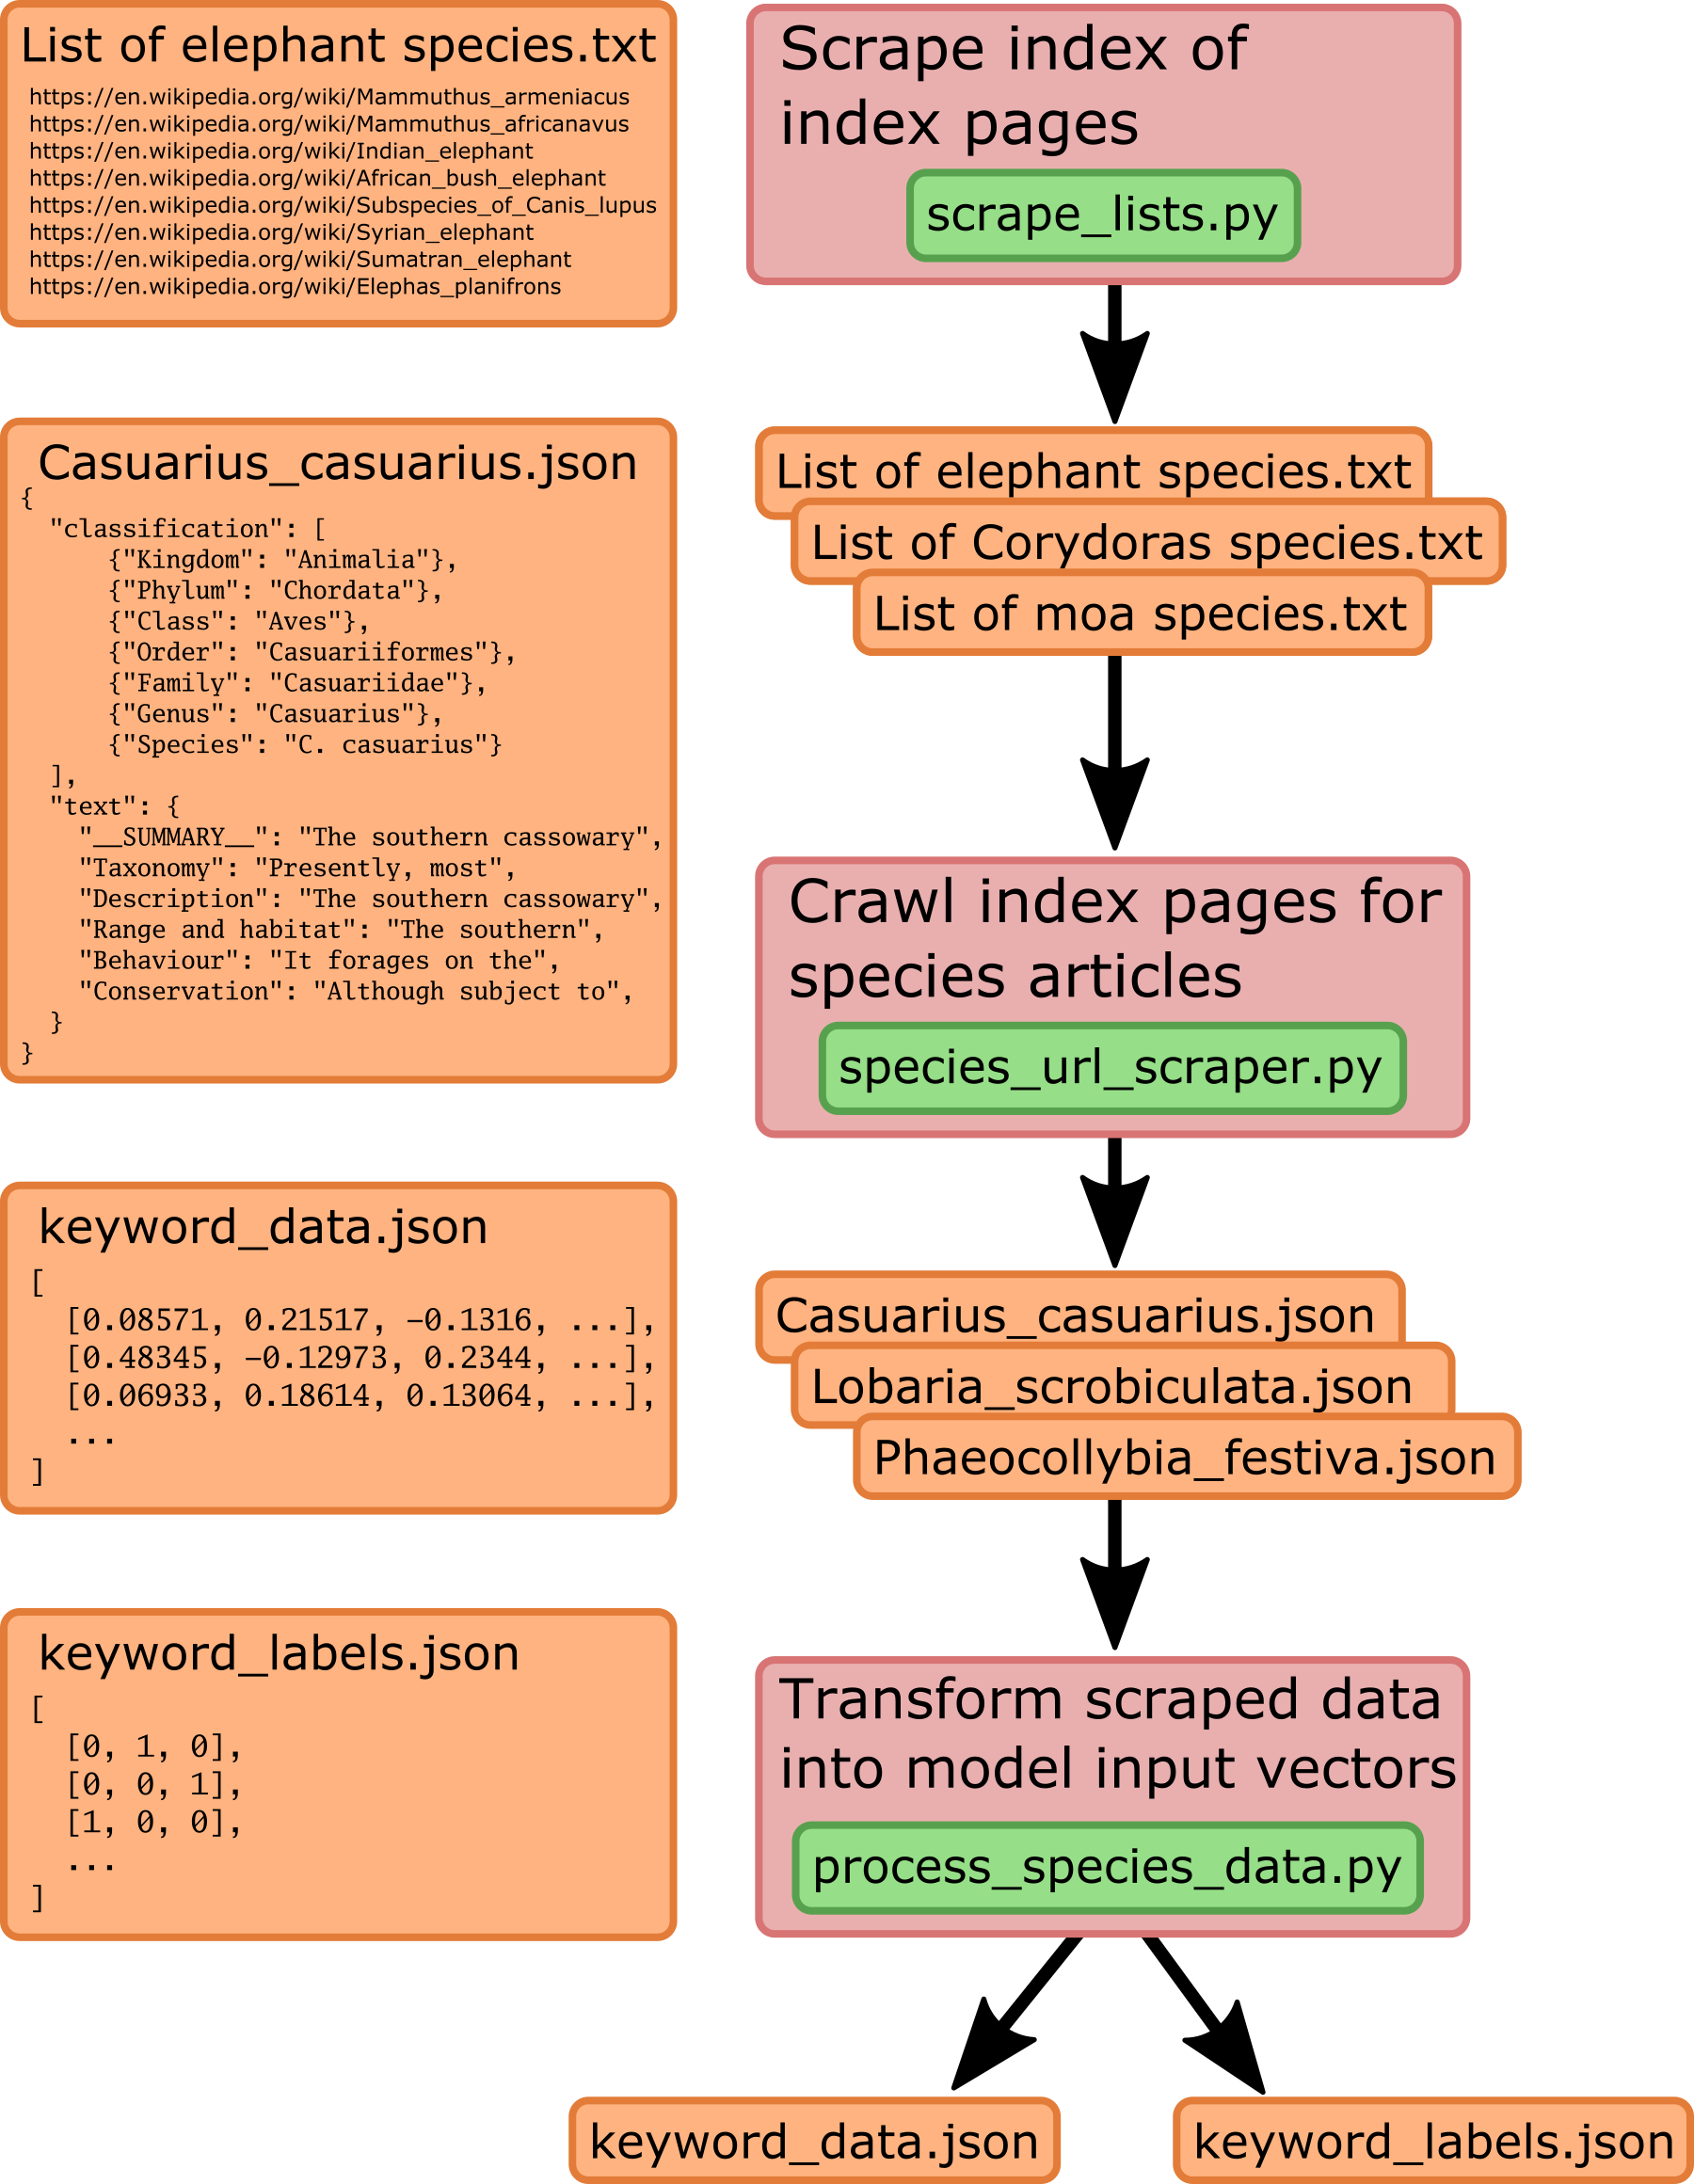
\includegraphics[width=\linewidth]{data.png}
  \caption{Visualization of the data-processing pipeline.}
  \label{fig:data}
\end{figure}

A flowchart of the data collection and processing pipeline can be seen in Figure \ref{fig:data}. The process involves collecting data from Wikipedia and then processing it into representations that will be used as inputs for the deep learning model.

We leveraged Python scripts for their simplicity and the availability of relevant libraries. 

\subsection{Scrape index pages}
The first step is to creates lists of species articles which is done by supplying manually-found species index pages using \texttt{species\_url\_scraper.py} which then scrapes these articles to output lists of Wikipedia article URLs. This scraping is done with an HTML parser that searches for hyperlinks that match the \texttt{https://en.wikipedia.org/wiki/Article} form. These are then checked to ensure they actually correspond to an organism. This step outputs a collection of URLs of these articles.

\subsection{Scrape species articles}
The next step consumes these URL lists and scrapes the Wikipedia pages to extract the scientific classification as well as the text content from each of the sections. The scraping parses the classification from the info boxes on the side of all the pages, which are very consistently-structured across all of English Wikipedia. The text content of various sections is retrieved reliably using the Wikipedia API.

\subsection{Create input vectors}
The final step of the data process involves loading all of the crawled data into memory to create our final training data and labels. We take the raw data and apply functions to create training data and training labels. We work with two different functions to create our data which is detailed in Section \ref{section:methods}.

\subsection{Review Collected Data}

We selected animal, plant, and fungi pages to scrape (we decided to not work with unicellular organisms simply because they are vastly different from multicellular ones). We ultimately collected data for 25474 species-level pages (5926 animal, 16574 plant, and 2974 fungi). 

We took a lot at our data by observing the sizes of key parts of the articles by plotting histograms as seen in Figure \ref{fig:article_lengths}. Every Wikipedia article has a "summary" which is the initial text without any particular header. There are many "stub" articles with very few words in the summary and little total content. An extremely common first section for species articles was "Description" (10070/25474 articles contained this section). Much like the summaries we note that there is a large number of small descriptions, but the large majority of descriptions are medium-to-large in length, a good sign that this data is going to be useful.

\begin{figure}
  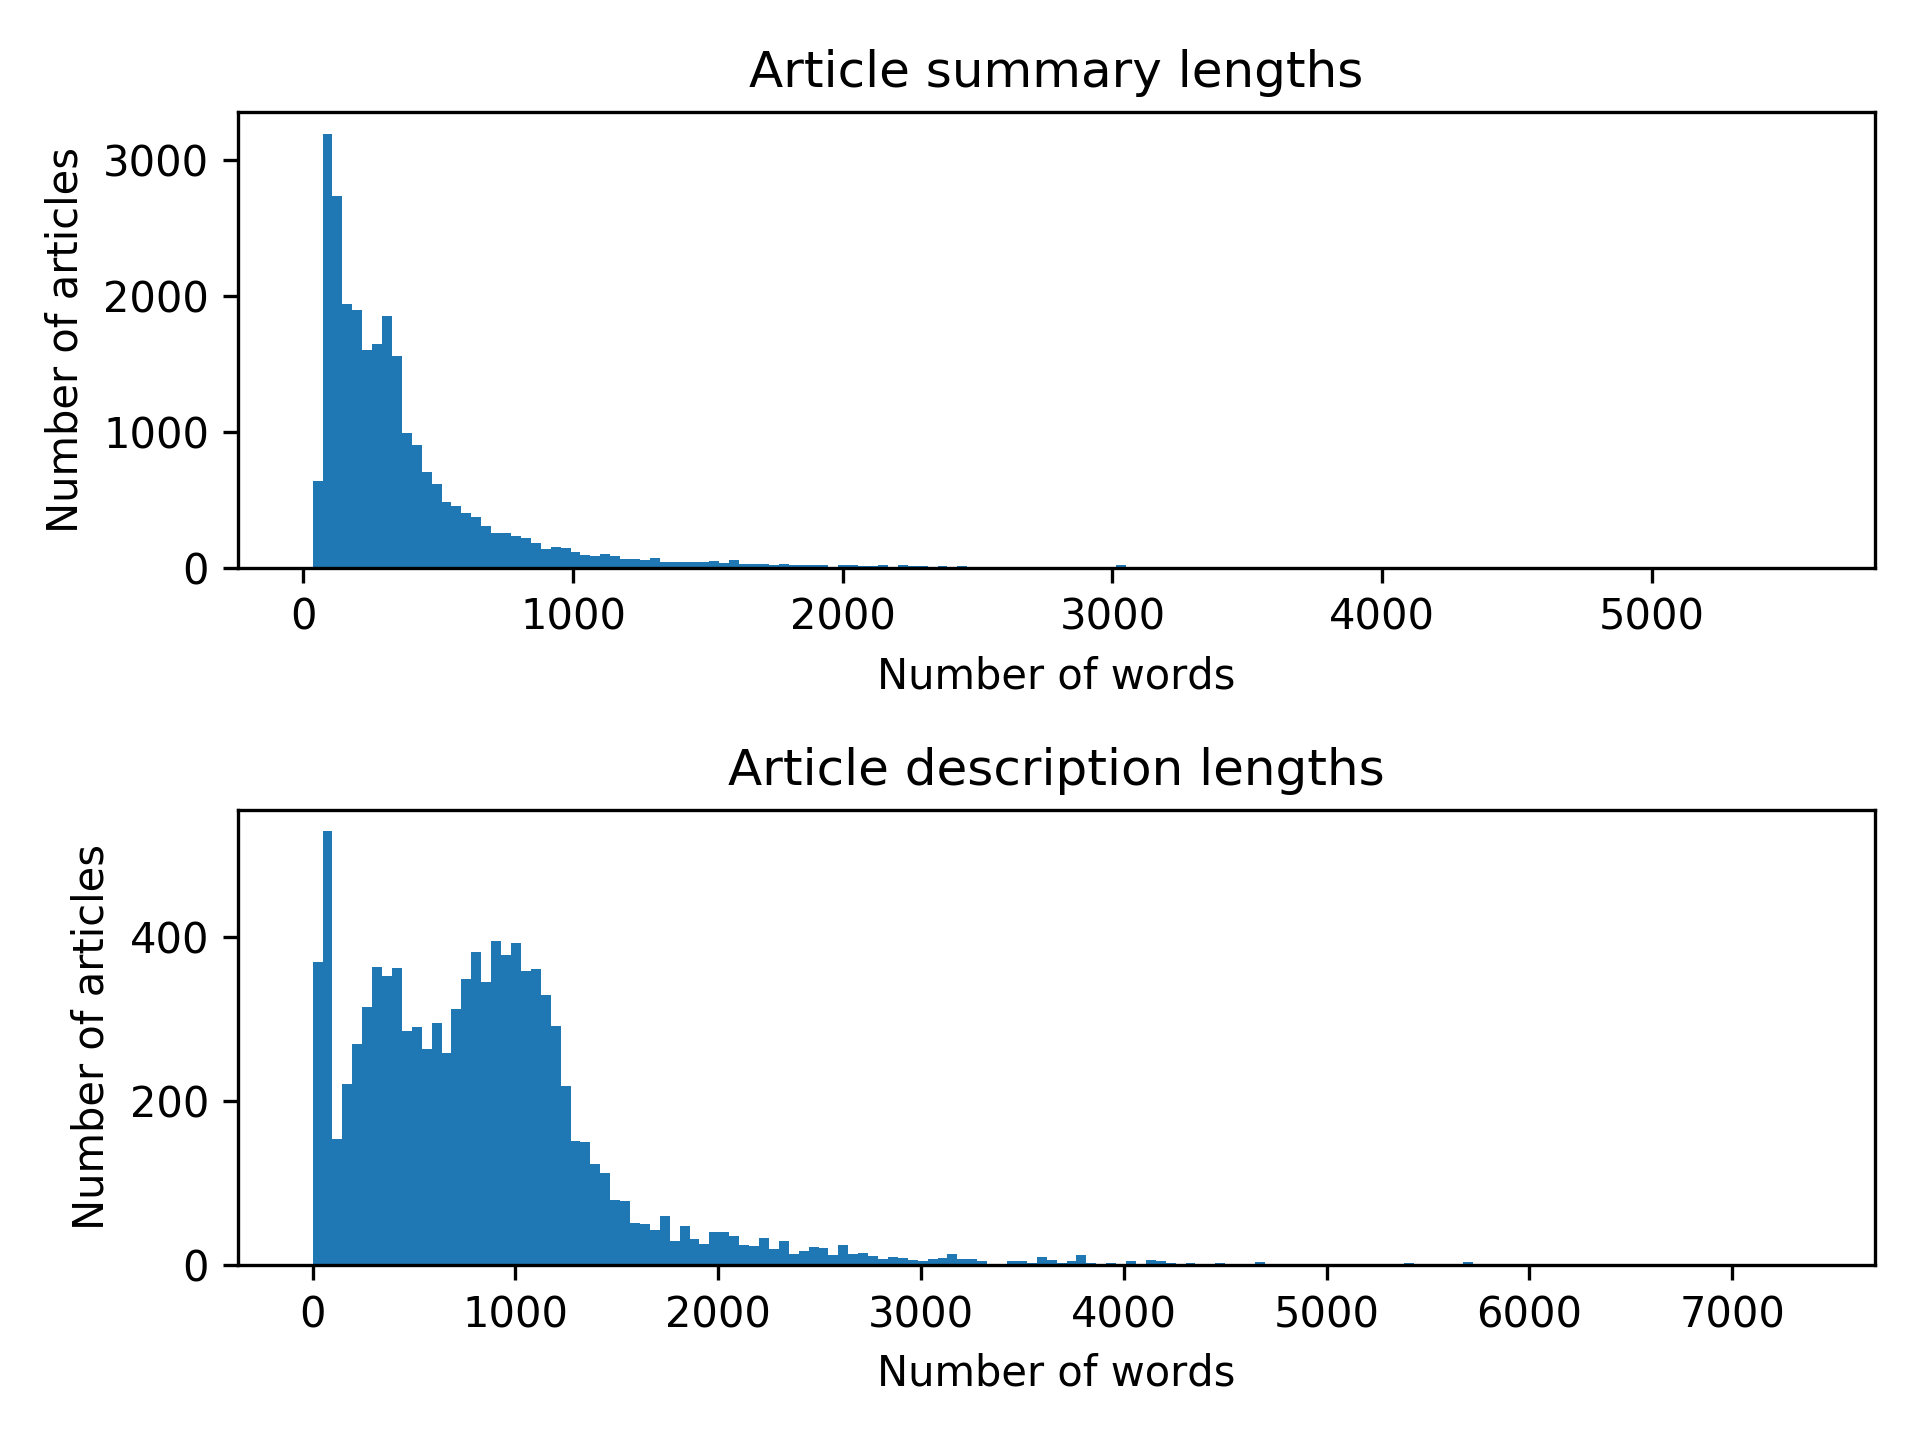
\includegraphics[width=\linewidth]{article_lengths.png}
  \caption{asdf}
  \label{fig:article_lengths}
\end{figure}

With more time, we would have liked to experiment with filtering on the data to remove articles with certain characteristics, for example we could filter a decent amount of articles with extremely short summaries or descriptions without. Filtering to only use articles that contain descriptions is another experiment that we hypothesize may improve results at the expense of discarding over half of the scraped articles. 

\section{Methods}
\label{section:methods}

Our classifier design can be seen in Figure \ref{fig:classifier_overview}. We decided to try two different natural language processing methods to generate representations of the data. The first was a simple keyword extractor followed by a pre-trained word embedding model. The other was BERT, the Bidirectional Encoder Representations from Transformers model by Google. These vectorized representations could then be easily fed into a feed forward model for training. For testing, we widtheld some of the testing data for cross validation and we attempted to write our own paragraphs to see if the model could predict the taxonomy we were thinking of. 
\begin{figure*}
  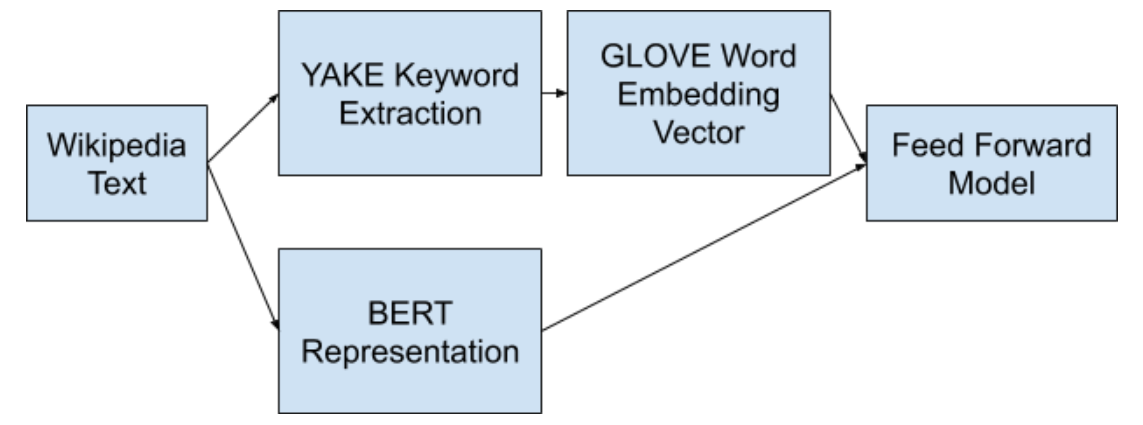
\includegraphics[width=\linewidth]{classifier_overview.png}
  \caption{Flowchart of our classifier.}
  \label{fig:classifier_overview}
\end{figure*}

\subsection{Keyword Extraction}
We decide to use YAKE, Yet Another Keyword Extractor by Campos et al. Using PKE, the Python Keyphrase Extraction module, we tested several keyword extractors and chose YAKE for its simplicity and proven success. We fed the pretrained model our wikipedia texts and it returned the top 20 keywords and their relevancy scores. 
\begin{figure*}
  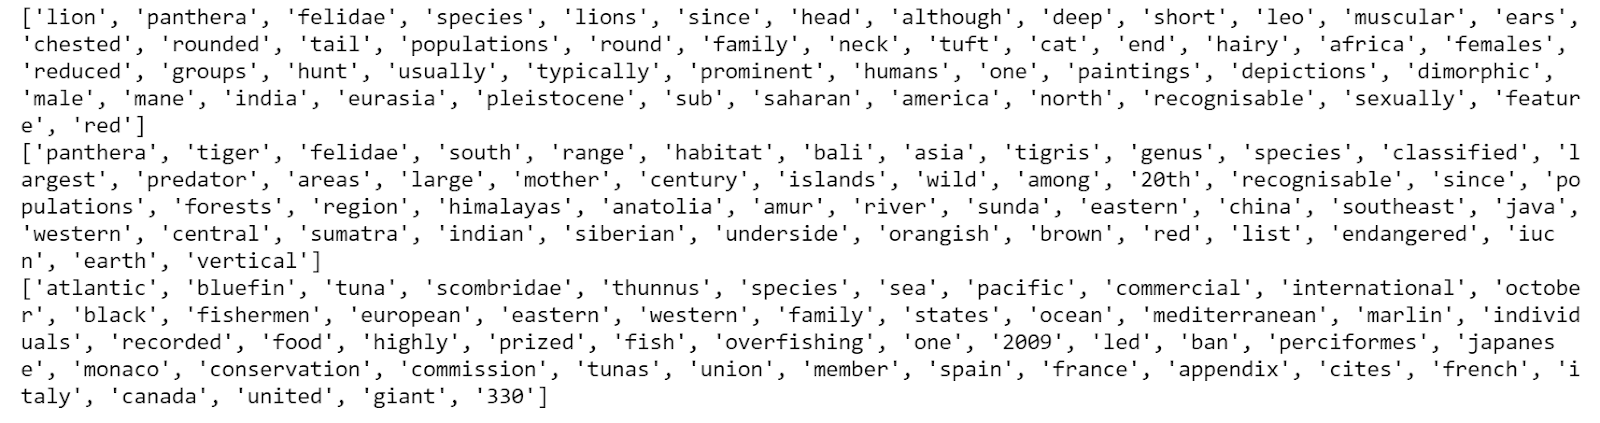
\includegraphics[width=\linewidth]{keywords_example.png}
  \caption{Examples of keywords extracted from the lion, tiger, and bluefin tuna wikipedia pages.}
  \label{fig:keywords_example}
\end{figure*}

To vectorize our keywords, we used the pre-trained word embeddings model, GloVe or Global Vectors for Word Representation. The model was pretrained on 2014 wikipedia data which made it suitable for representing our input. In testing, we discovered some words in our data had not been seen by GloVe and we were unable to vectorize it. We decided to remove those words from our training data because it rarely occurred and the pretrained model was able to generate vectors for most of our keywords. A possible alternative would be to train our own GloVe model based on the data we have. 

After vectorizing the keywords, we used a weighted sum of the vectors based on their relevancy scores. Our first attempt to directly sum the vectors resulted in vectors that were all very similar to each other. We attribute this to some common words that are irrelevant to species taxonomy pushing the vectors in a common direction since most wikipedia descriptions use similar language. Our weighted sum approach seemed to overcome this. We multiplied the keyword vectors by its relevancy scores scaled. In other words, the sum of the relevancy scores equalled 1. As a result of this however, our representation varied from the GloVe representation and applying the word embeddings map in the other direction gave irrelevant results. However, from testing different animal species, we saw a good correlation between similar species. As an example, using Euclidean distance as our distance metric, we found that the Lion vector was close to the Tiger vector, but both were far from Bluefin Tuna. This result led us to believe that we have successfully created a representation that stores the characteristics associated with different species. 


\section{Experiments}

These are the experiments.

\section{Results}

These are the results.

\section{Conclusions}

This is wonderful.

{\small
\bibliographystyle{ieee}
\bibliography{bibliography}
}

\end{document}
